\documentclass[twocolumn]{article}
\setlength{\columnsep}{0.25in}
\usepackage[utf8]{inputenc}
\usepackage[margin=1in]{geometry}
\usepackage{times}
\usepackage{amssymb}
\usepackage{amsmath}
\usepackage{graphicx}
\usepackage{textcomp}
\usepackage{multirow}
\usepackage[T1]{fontenc}

\usepackage{biblatex}
\addbibresource{refs.bib}

\renewcommand{\ttdefault}{zlmtt}

\title{\textbf{Supervised Classification of Twitter Data}}
\author{
    Shrey Desai \\
    \texttt{shreydesai@utexas.edu}
}
\date{}

\begin{document}

\maketitle

\section{Introduction}

Document classification, the assignment of documents to one or more classes or categories, remains an important problem in computer science and natural language processing. While much research has focused on analyzing large documents, such as books and product reviews, short documents have not been investigated to the same degree. Twitter offers a unique platform for the analysis of short text documents -- a user’s “tweet” is restricted to 140 characters. In this project, we explore the classification of tweets into the categories of entertainment, fun, games, politics, science, sports, technology, and weather, using supervised methods.

Currently, Twitter does not support the broad search of tweets according to genre. While users can find tweets consisting of a specific substring, hashtag, or mention, they are unable to find a set of tweets pertaining to the genre searched for. For example, the query ``news'' returns tweets strictly containing the substring ``news'' or the hashtag ``\#news.'' However, it does not yield a set of news-related tweets from reputable accounts such as the NY Times, Huffington Post, and TechCrunch.

The motivation for this project is therefore to explore how such a system could be built. Provided that our classification system is accurate and scalable, users would be able to subscribe to different topics and receive a personalized feed of tweets from said categories. Since hashtags are not always accurate and can be misleading, this system could also aid information retrieval tasks that need to fetch tweets from a specific category.

\section{Methods}

\subsection{Retrieval}

For each of the 8 categories, we compiled a handpicked list of 20 users that commonly tweet within that category. For example, we would expect the Weather Channel to tweet about weather-related news and the Olympics to tweet about sports events. After a complete list of 160 users was compiled, approximately 3000 tweets were downloaded from user. In order to avoid using too much memory, these tweets were grouped by category and stored in a directory for future analysis. See \S{3} for a detailed discussion on the corpus selection and construction process.

\subsection{Preprocessing}

Raw Twitter data is not suitable to build a corpus because of its variability in structure and content. The preprocessing phase consists of filtering tweets that do not meet certain guidelines and removing tokens that might interfere with the classification step.

First, retweets (\texttt{RT <content>}) and tweets that start with a mention (\texttt{@<username>}) are automatically excluded. Retweets and mentions often take the form of comments to other users, so they do not fit well within a single category. Both of these types of tweets are filtered through regular expressions, where the pattern matches the \texttt{RT} and \texttt{@}, respectively.

Second, links and non-ASCII characters (emojis) are removed from tweets. Links are detected with a regular expression that matches Twitter’s unique URL shortener, \texttt{t.co}. For non-ASCII characters, we use a set of ASCII characters and check whether the characters in a token form a subset of this set.

Third, we maintain a set of tweets within each category that have been processed. This ensures that duplicate tweets are not added into the corpus.

\subsection{Classification}

In order to classify the tweets, we use three different classifiers from the \texttt{scikit-learn} \cite{scikit} package – Multinonial Naive Bayes (\texttt{MultinomialNB}), Support Vector Machine (\texttt{NuSVC}), and Logistic Regression (\texttt{LogisticRegression}). We use various feature sets for the classifiers, including unigrams, bigrams, POS unigrams, POS bigrams, and a combination of all four. Using our processed tweets as our corpus, the training set takes 70\% of the corpus and the test set takes 30\%.

\section{Corpora}

As alluded to previously, we are using Twitter to build our corpus. The corpus consists of tweets from 8 categories -- \textit{entertainment}, \textit{fun}, \textit{games}, \textit{politics}, \textit{politics}, \textit{science}, \textit{sports}, \textit{technology}, and \textit{weather}. Below is a brief description of what kinds of tweets would be included in each category:
\begin{itemize}
    \itemsep 0em
    \item \textit{Entertainment} -- TV, Hollywood, social media
    \item \textit{Fun} -- Humor, sarcastic remarks, Internet memes
    \item \textit{Games} -- PC/Console games, video game culture
    \item \textit{Politics} -- Elections, government officials/agencies
    \item \textit{Science} -- Research, scientific facts, global warming
    \item \textit{Sports} -- News from the NFL, NBA, MLB, etc.
    \item \textit{Technology} -- Tech gadgets, data science, programming, privacy and security
    \item \textit{Weather} -- Forecast, storm updates, flood warnings
\end{itemize}

In order to collect tweets from each category, we make the assumption that there are certain Twitter accounts that, for the most part, tweet about topics within that category. For example, we would include the Olympics as an account in the sports category, but we would not include Jimmy Kimmel in the fun category because he has a potential to tweet about other topics as well, such as politics, entertainment, and possibly technology.

Twitter offers a public API that allows developers to download public tweets from any user. We created a list of 20 user handles from each category -- with 160 user handles total -- and retrieved tweets from each one. Because of Twitter's API rate limits, we have only been able to collect around 3000 recent tweets from each user.

Below is a table showing the breakdown of our corpus. The unprocessed column shows how many raw tweets were retrieved in each category. The processed column shows how many tweets remain for classification after filtering and cleaning.

\begin{table}[h]
\centering
\caption{Twitter Data Corpus}
\begin{tabular}{|l|l|l|}
\hline
\multicolumn{1}{|c|}{\textbf{Category}} & \multicolumn{1}{c|}{\textbf{Unprocessed}} & \multicolumn{1}{c|}{\textbf{Processed}} \\ \hline
Entertainment                           & 64574                                     & 46394                                   \\ \hline
Fun                                     & 62603                                     & 38830                                   \\ \hline
Games                                   & 64439                                     & 46737                                   \\ \hline
Politics                                & 64595                                     & 43354                                   \\ \hline
Science                                 & 63969                                     & 46082                                   \\ \hline
Sports                                  & 64550                                     & 40200                                   \\ \hline
Technology                              & 64037                                     & 42912                                   \\ \hline
Weather                                 & 64484                                     & 39101                                   \\ \hline
\end{tabular}
\end{table}

\section{Features}

\subsection{Unigrams}

Individual words formed a good baseline indicator of what sorts of words were included in each category. Common stopwords, such as ``the,'' ``of,'' ``and,'' and ``is'' were not removed from the sentences. The tweets were already small enough to begin with, so removing more words would had a negative impact on classification. Figure 7 shows the most frequent unigrams in each category, excluding stopwords.

\subsection{Bigrams}

We used NLTK's \texttt{BigramCollocationFinder} to form bigrams from sentences. The resulting bigrams were selected using a Chi Squared test (\texttt{BigramAssocMeasure.ch\_sq}), which found the most informative bigrams relative to each category. Figure 8 shows the most frequent bigrams in each category, excluding stopwords.

\subsection{Part of Speech (POS)}

POS tags such as nouns, verbs, adjectives, and adverbs gave more information on how words were being used in the sentences. We hypothesized that there might be certain words used as different POS tags which might be useful during classification. The NLTK \texttt{UnigramTagger}, trained on the Brown corpus, was used to tag the tweets. Finally, we considered both POS unigrams and bigrams; each had a feature set that was given to the classifiers.

\begin{figure}
    \centering
    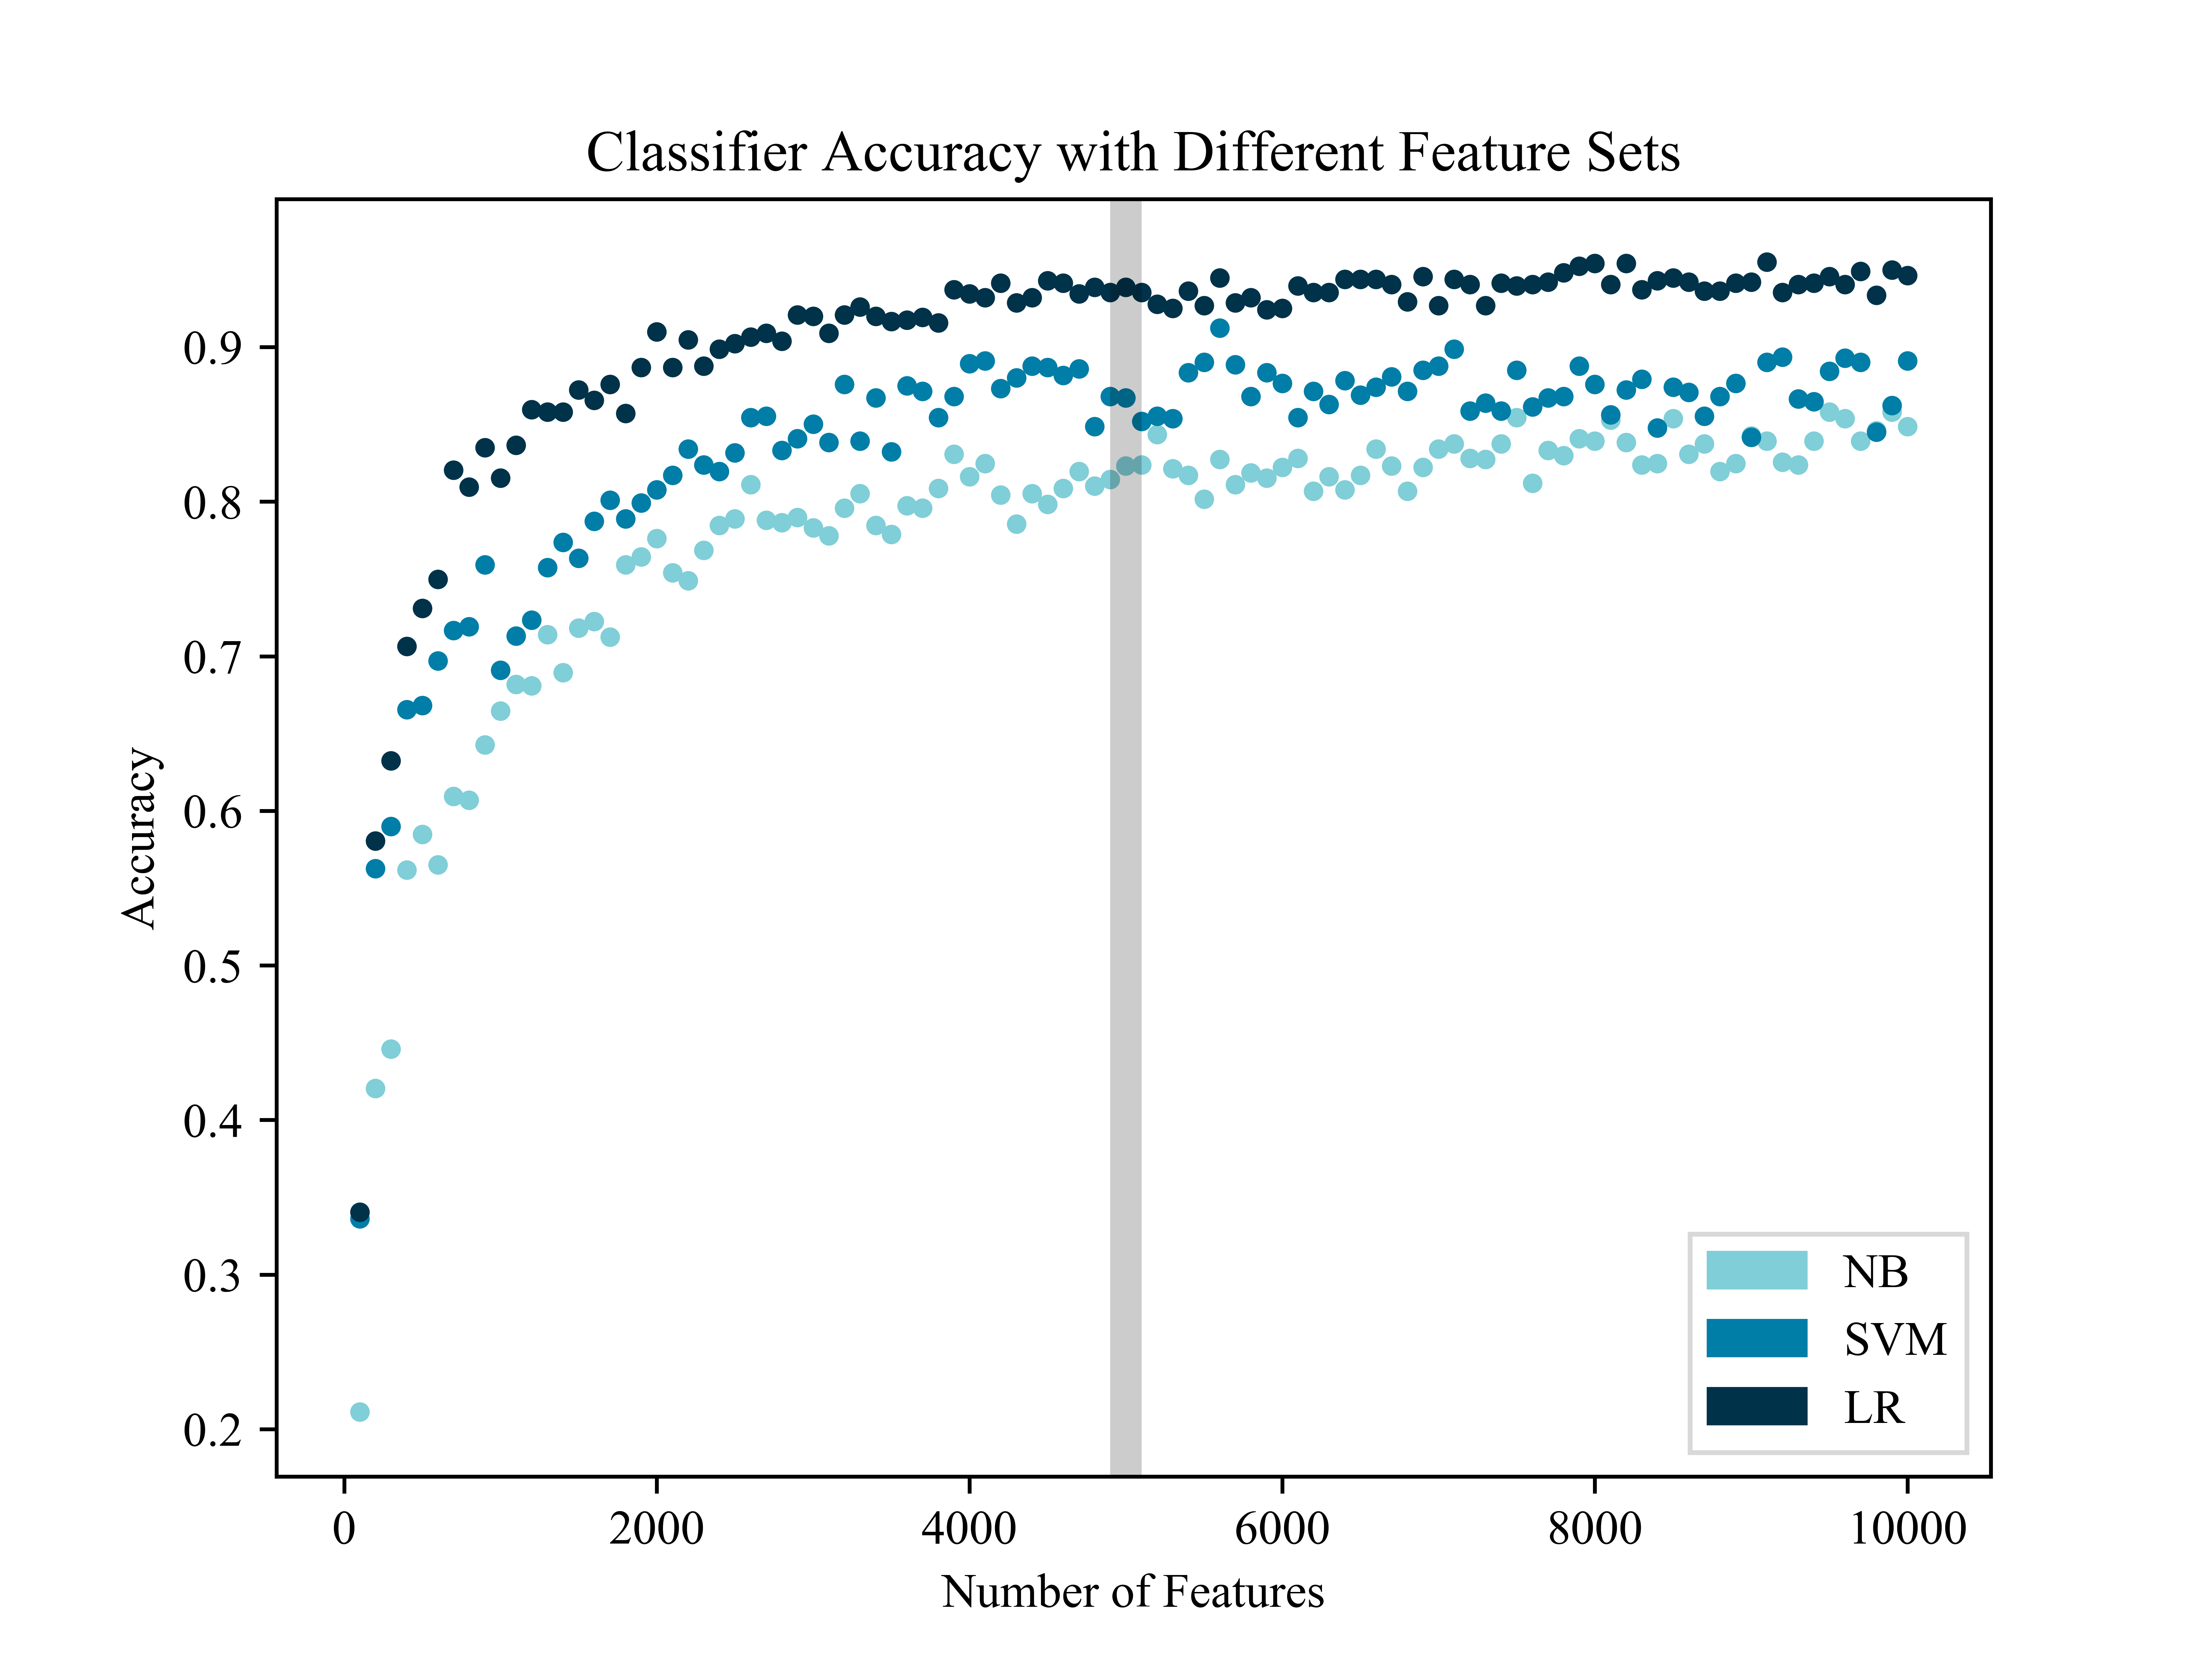
\includegraphics[width=8cm]{iter_accuracy}
    \caption{Effect of Feature Set Size on Accuracy}
\end{figure}

\section{Experiments}

There were five feature sets that were constructed for the classifiers -- unigrams, bigrams, POS unigrams, POS bigrams, and a combination of all features. For each experiment, each classifier was run 50 times with its respective feature set. The final accuracy value was an average over each accuracy value recorded during an iteration. Table 2 shows the results for each experiment. The Naive Bayes, Support Vector Machine, Logistic Regression, and Standard Deviation are abbreviated as NB, SVM, LR, and Std Dev, respectively.

\begin{table}[h]
\centering
\caption{Experiment Results}
\begin{tabular}{|c|l|l|l|}
\hline
\textbf{Experiment}           & \multicolumn{1}{c|}{\textbf{Classifier}} & \multicolumn{1}{c|}{\textbf{Accuracy}} & \multicolumn{1}{c|}{\textbf{Std Dev}} \\ \hline
\multirow{3}{*}{Unigram}      & NB                                       & 81.74\%                                & 0.07108                           \\ \cline{2-4}
                              & SVM                                      & 85.91\%                                & 0.0421                            \\ \cline{2-4}
                              & LR                                       & 91.65\%                                & 0.03151                           \\ \hline
\multirow{3}{*}{Bigram}       & NB                                       & 93.02\%                                & 0.03324                           \\ \cline{2-4}
                              & SVM                                      & 58.96\%                                & 0.16244                           \\ \cline{2-4}
                              & LR                                       & 90.97\%                                & 0.04351                           \\ \hline
\multirow{3}{*}{POS Unigram}  & NB                                       & 53.78\%                                & 0.06411                           \\ \cline{2-4}
                              & SVM                                      & 53.87\%                                & 0.05389                           \\ \cline{2-4}
                              & LR                                       & 54.46\%                                & 0.06254                           \\ \hline
\multirow{3}{*}{POS Bigram}   & NB                                       & 56.68\%                                & 0.06059                           \\ \cline{2-4}
                              & SVM                                      & 57.02\%                                & 0.06092                           \\ \cline{2-4}
                              & LR                                       & 58.04\%                                & 0.05958                           \\ \hline
\multirow{3}{*}{All Features} & NB                                       & 83.1\%                                 & 0.07326                           \\ \cline{2-4}
                              & SVM                                      & 87.95\%                                & 0.0431                            \\ \cline{2-4}
                              & LR                                       & 93.61\%                                & 0.03068                           \\ \hline
\end{tabular}
\end{table}

We were also curious to see whether changing the size of the feature set would affect classifier accuracy. Using a unigram feature set, we ran each classifier 50 times and recorded the average accuracy value. Figure 1 and 2 show how feature set size affected accuracy and training time, respectively. The gray interval in both graphs indicates the feature set size that we used in the previous experiments.

\begin{figure}
    \centering
    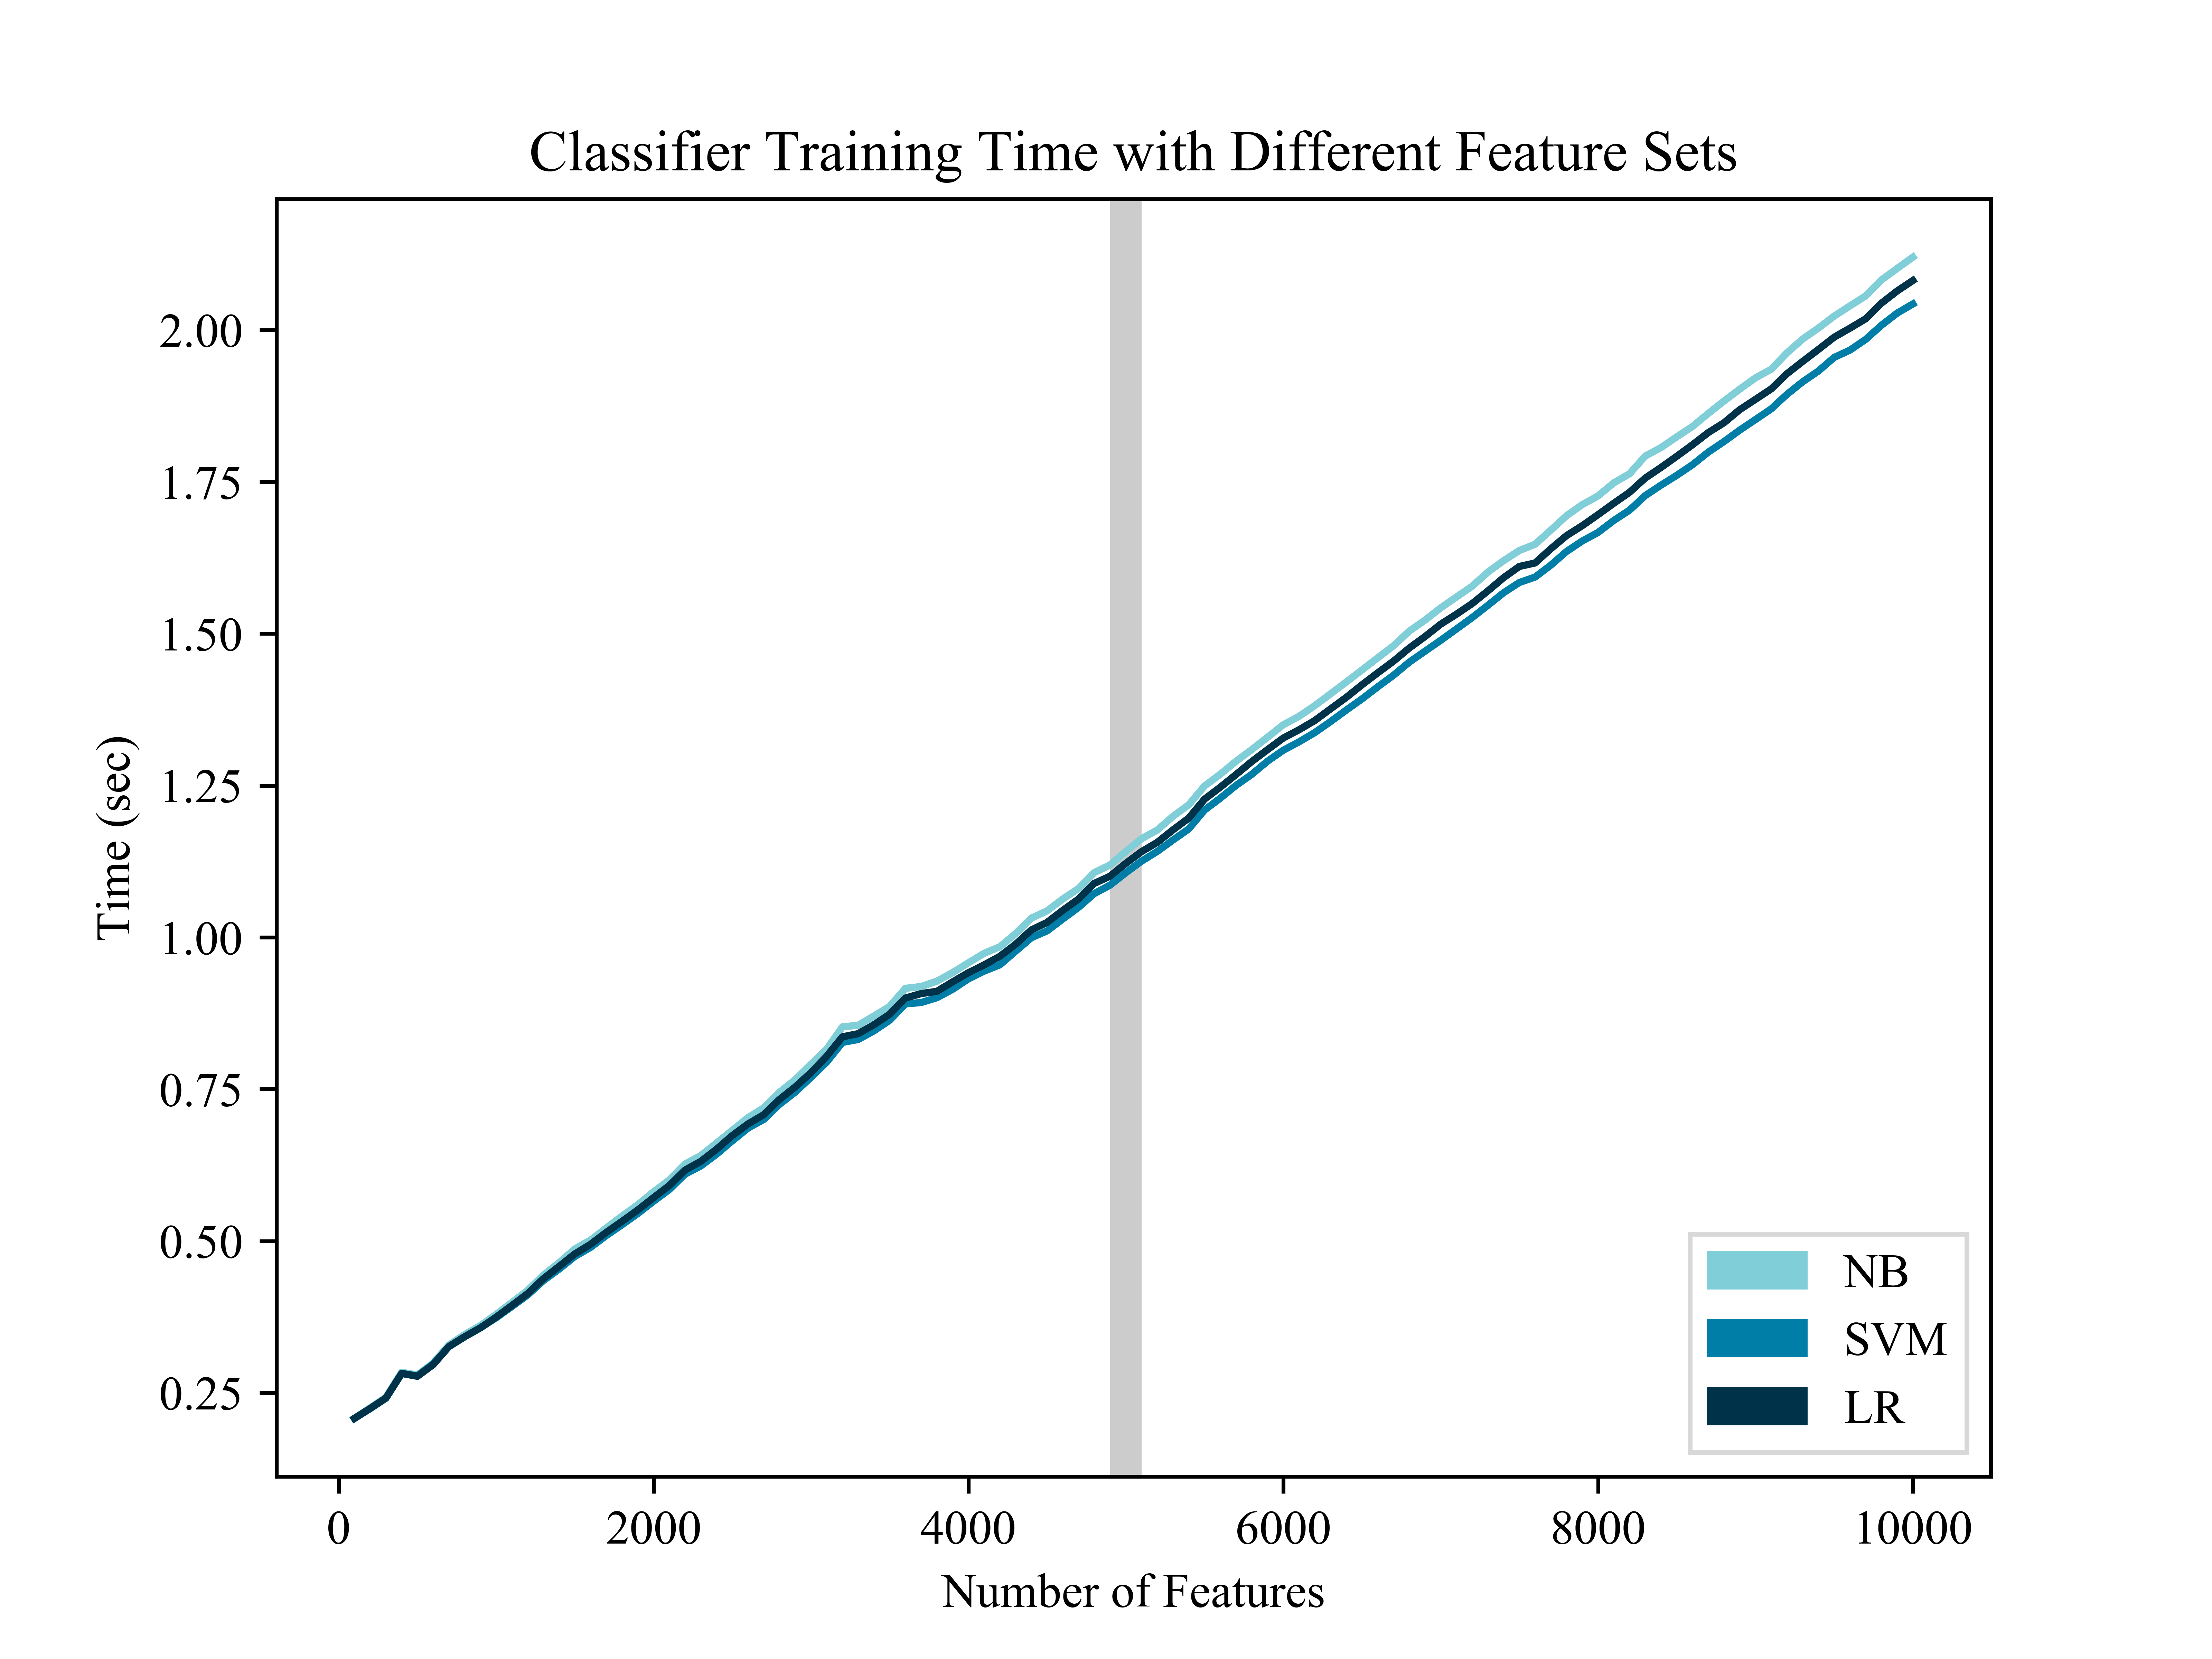
\includegraphics[width=8cm]{iter_time}
    \caption{Effect of Feature Set Size on Training Time}
\end{figure}

\section{Discussion}

\subsection{Classifier Accuracy}

The classifiers performed relatively well given a unigram feature set, which was used as a starting point for further improvement. With bigram features, the Naive Bayes classifier did exceptionally well but there was a reduction in accuracy for the SVM and Logistic Regression classifiers.

The low accuracies for the POS unigram and bigram feature sets was expected. The classification accuracy is highly contingent on the POS tagger accuracy. For instance, if most of the words in a sentence are labeled as nouns (NN), then the classifier will not have unique ways to disambiguate tweets. The NLTK \texttt{UnigramTagger} itself had around 45-50\% accuracy, so this likely affected the classification step.

The combination of all features (unigram, bigram, POS unigram, POS bigram) increased the accuracy of all classifiers in comparison to the baseline accuracy (unigram features). Figure 3 shows a side by side comparison of all feature sets and classifier performance. Finally, using a paired t-test (p < 0.05), we found that the improvement in accuracy from the baseline (unigram features) to the combined (all features) feature set was statistically significant for the SVM (p = 0.035) and Logistic Regression (p = 0.005) classifiers, but not the Naive Bayes (p = 0.332) classifier.

\begin{figure}
    \centering
    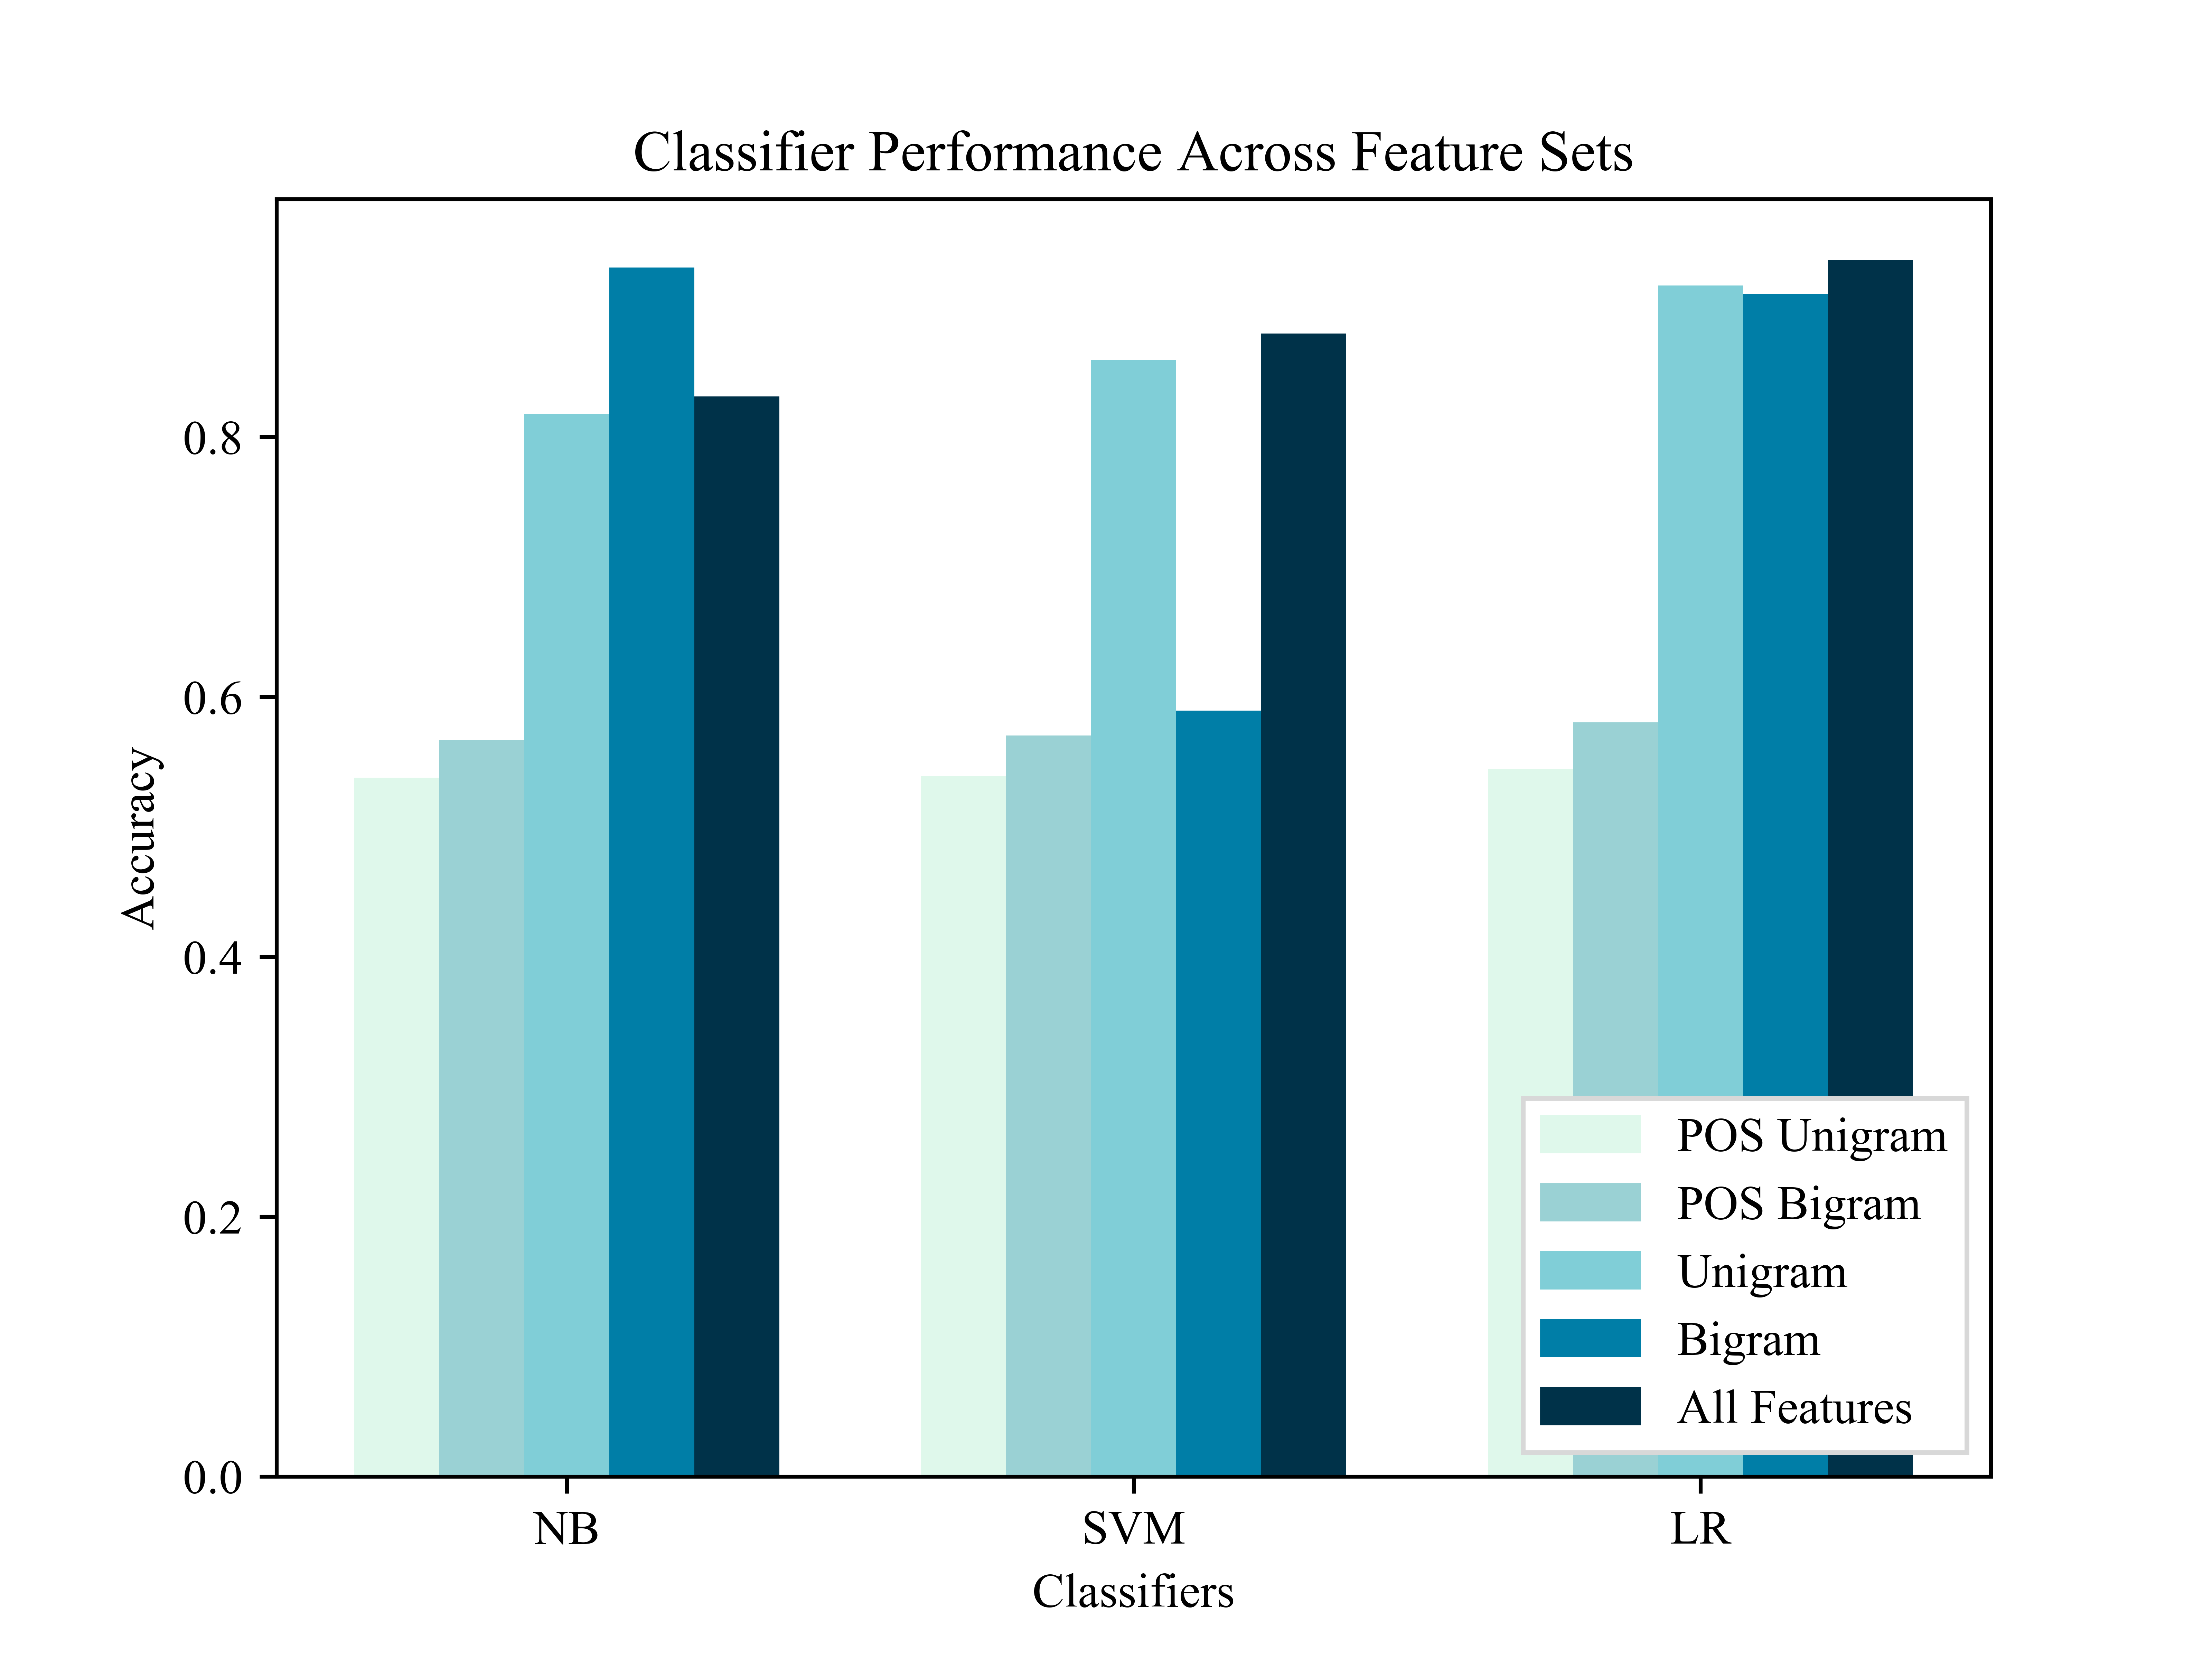
\includegraphics[width=8cm]{performance}
    \caption{Comparison of Different Feature Sets}
\end{figure}

\subsection{Feature Set Size}

Changing the size of the feature set did not have a huge impact on accuracy. Classifier accuracy improved drastically in the 0-2000 size interval, but it mostly leveled off as the size reached 10000. However, the time taken to train the classifiers increased linearly, taking around 2 seconds to train each classifier with 10000 features. With this data in mind, we decided on a feature set size of 5000 as it had decent accuracy and training time.

\subsection{Error Analysis}

To further analyze what each classifier got right and wrong, a confusion matrix across all 8 categories was generated. The matrix's diagonal shows the percentage of times the classifier made a correct prediction, while squares outside of the diagonal show the percentage of times the classifier was ``confused'' between those two categories and made an incorrect prediction. Figure 4, 5, and 6 display the matrix for the NB, SVM, and LR classifiers, respectively. Below are some observations from these matrices:
\begin{itemize}
    \itemsep 0em
    \item Naive Bayes was primarily unable to distinguish between entertainment/games and science/weather, where the error was made 6.4\% of the time. This makes sense because there are a lot of overlapping words between these categories. Games could be considered a form of entertainment and the weather is a subset of science.
    \item SVM made 4 errors, all 2.1\% of the time, which was better than Naive Bayes’ performance. It made a strange error by mixing up weather and games – perhaps the classifier mixed up a video game that was named after weather-related terms.
    \item Logistic Regression only made 2 errors, also both 2.1\% of the time. It is interesting how all three classifiers made an incorrect decision between entertainment/technology. There might have been significant overlap between those two categories for this error to be that widespread.
\end{itemize}

\begin{figure}
    \centering
    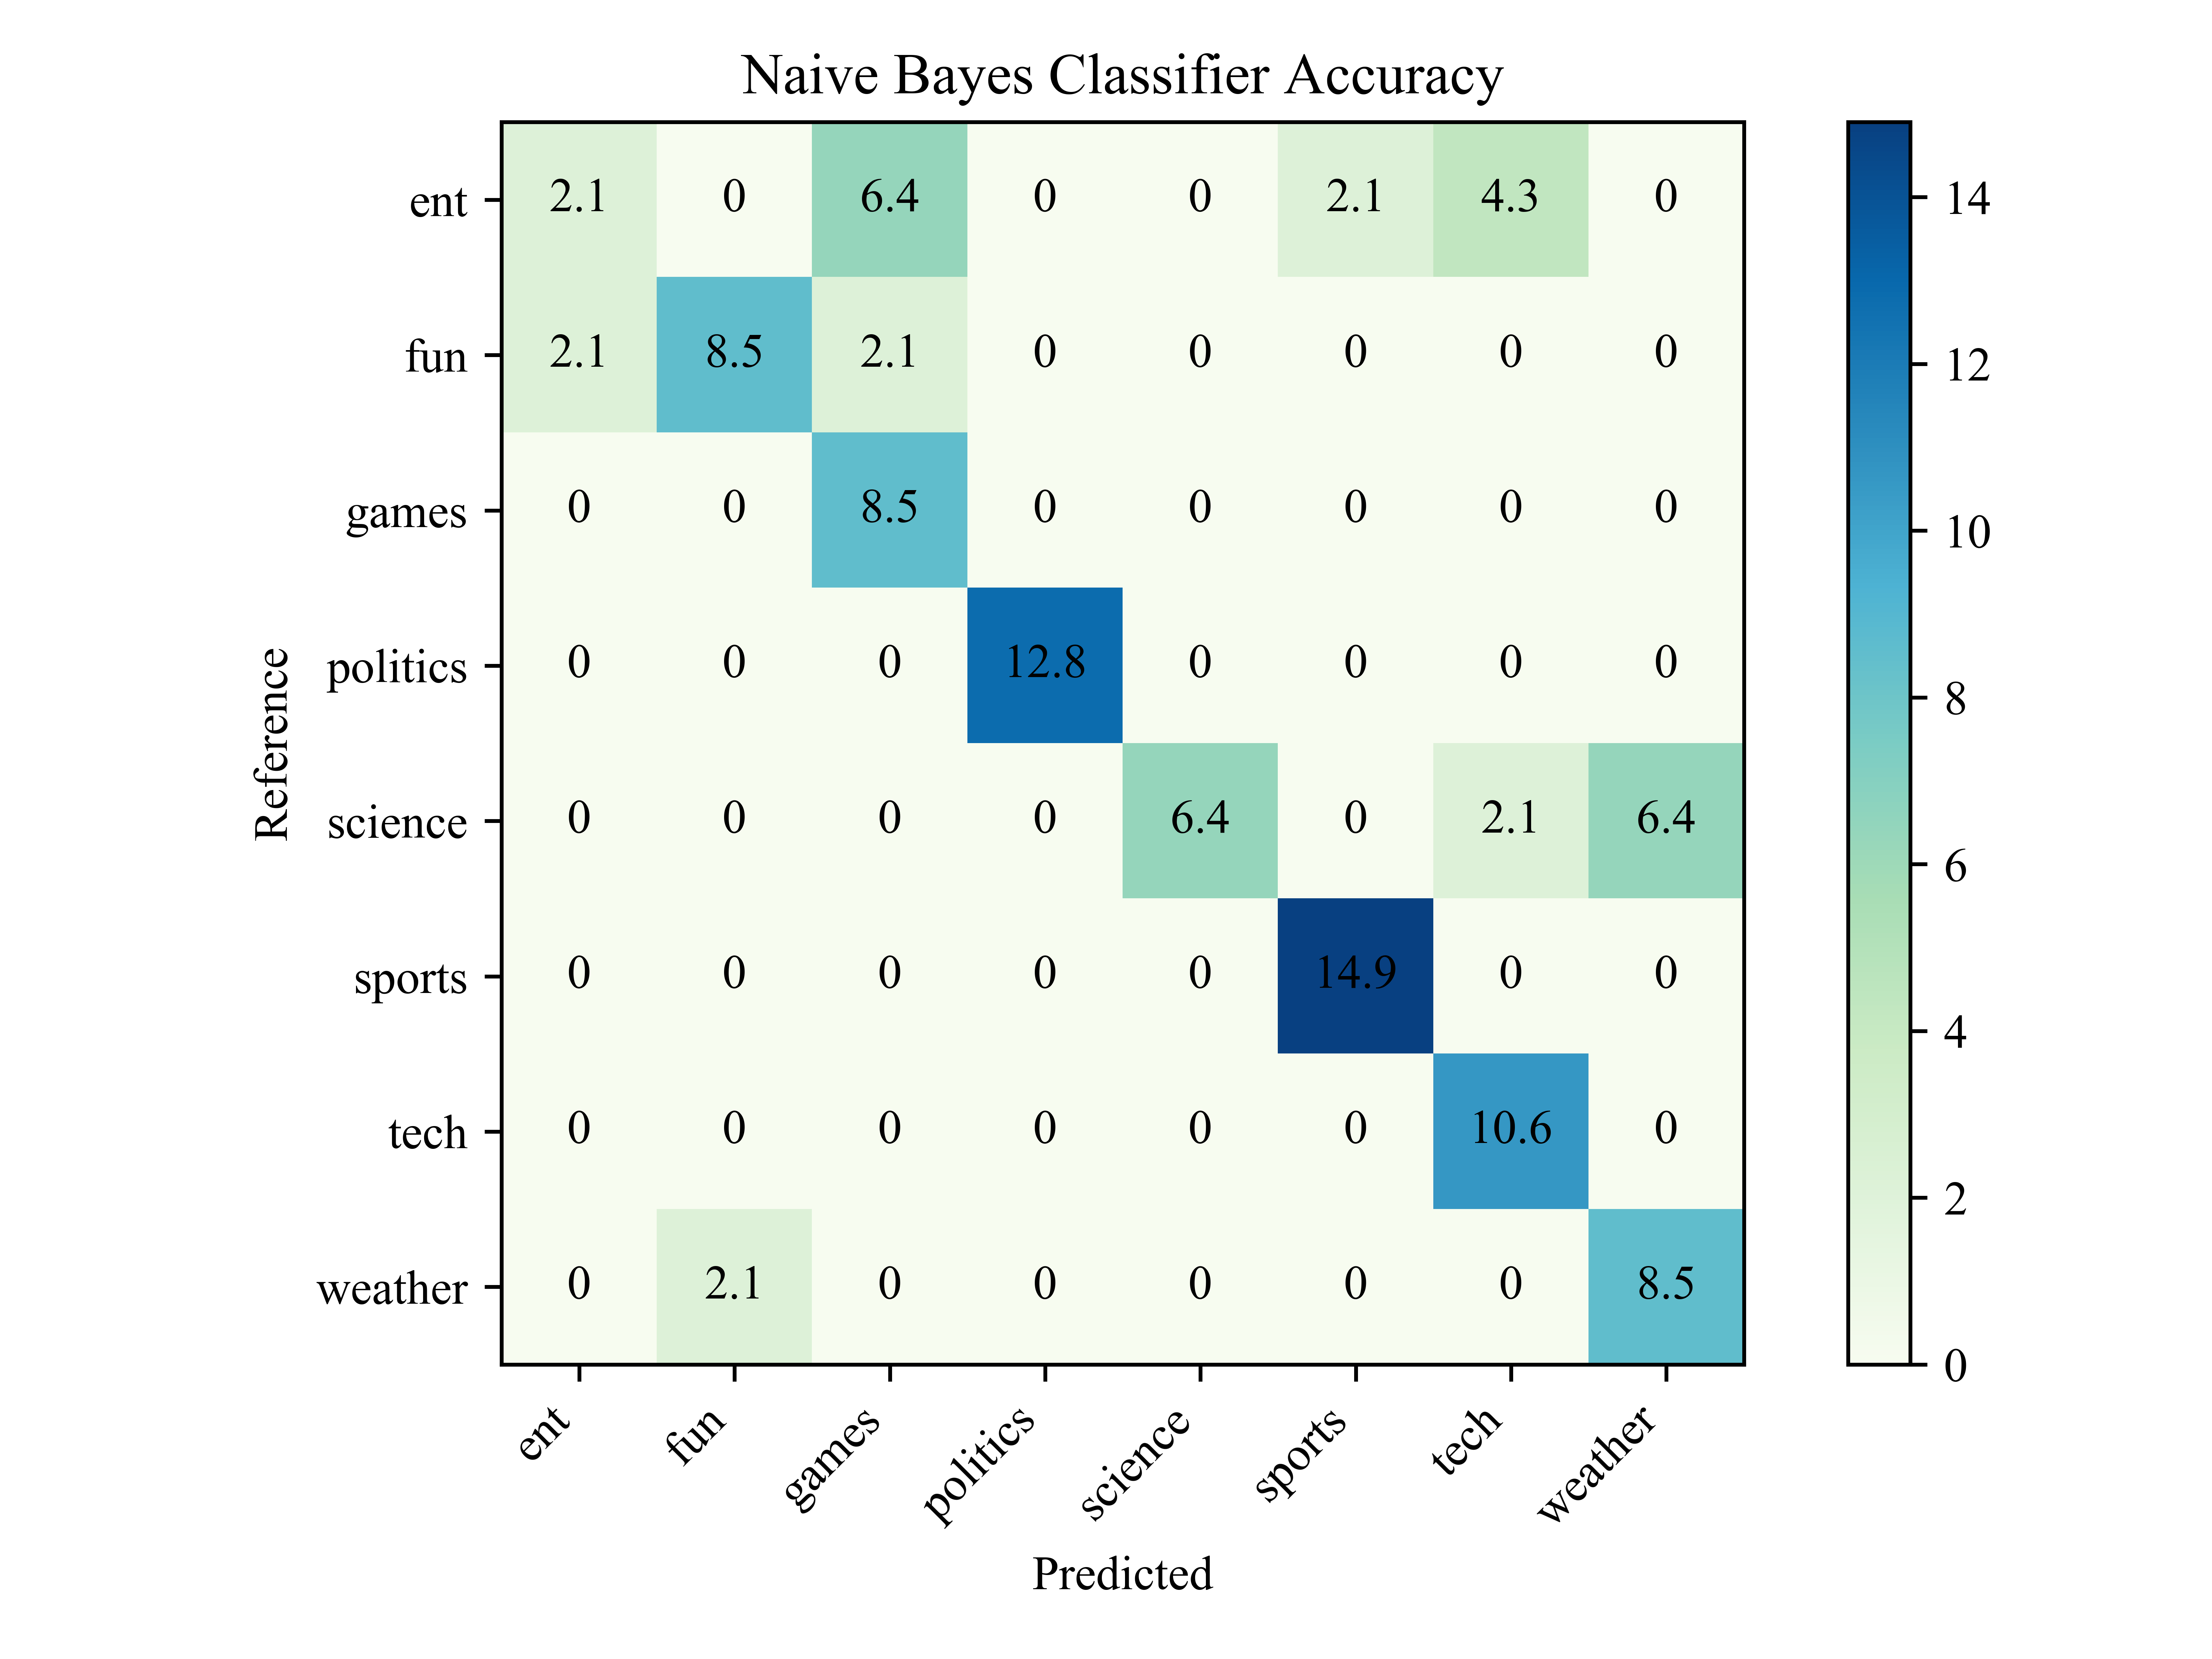
\includegraphics[width=8cm]{nb_cm}
    \caption{Naive Bayes Confusion Matrix}
\end{figure}

\begin{figure}
    \centering
    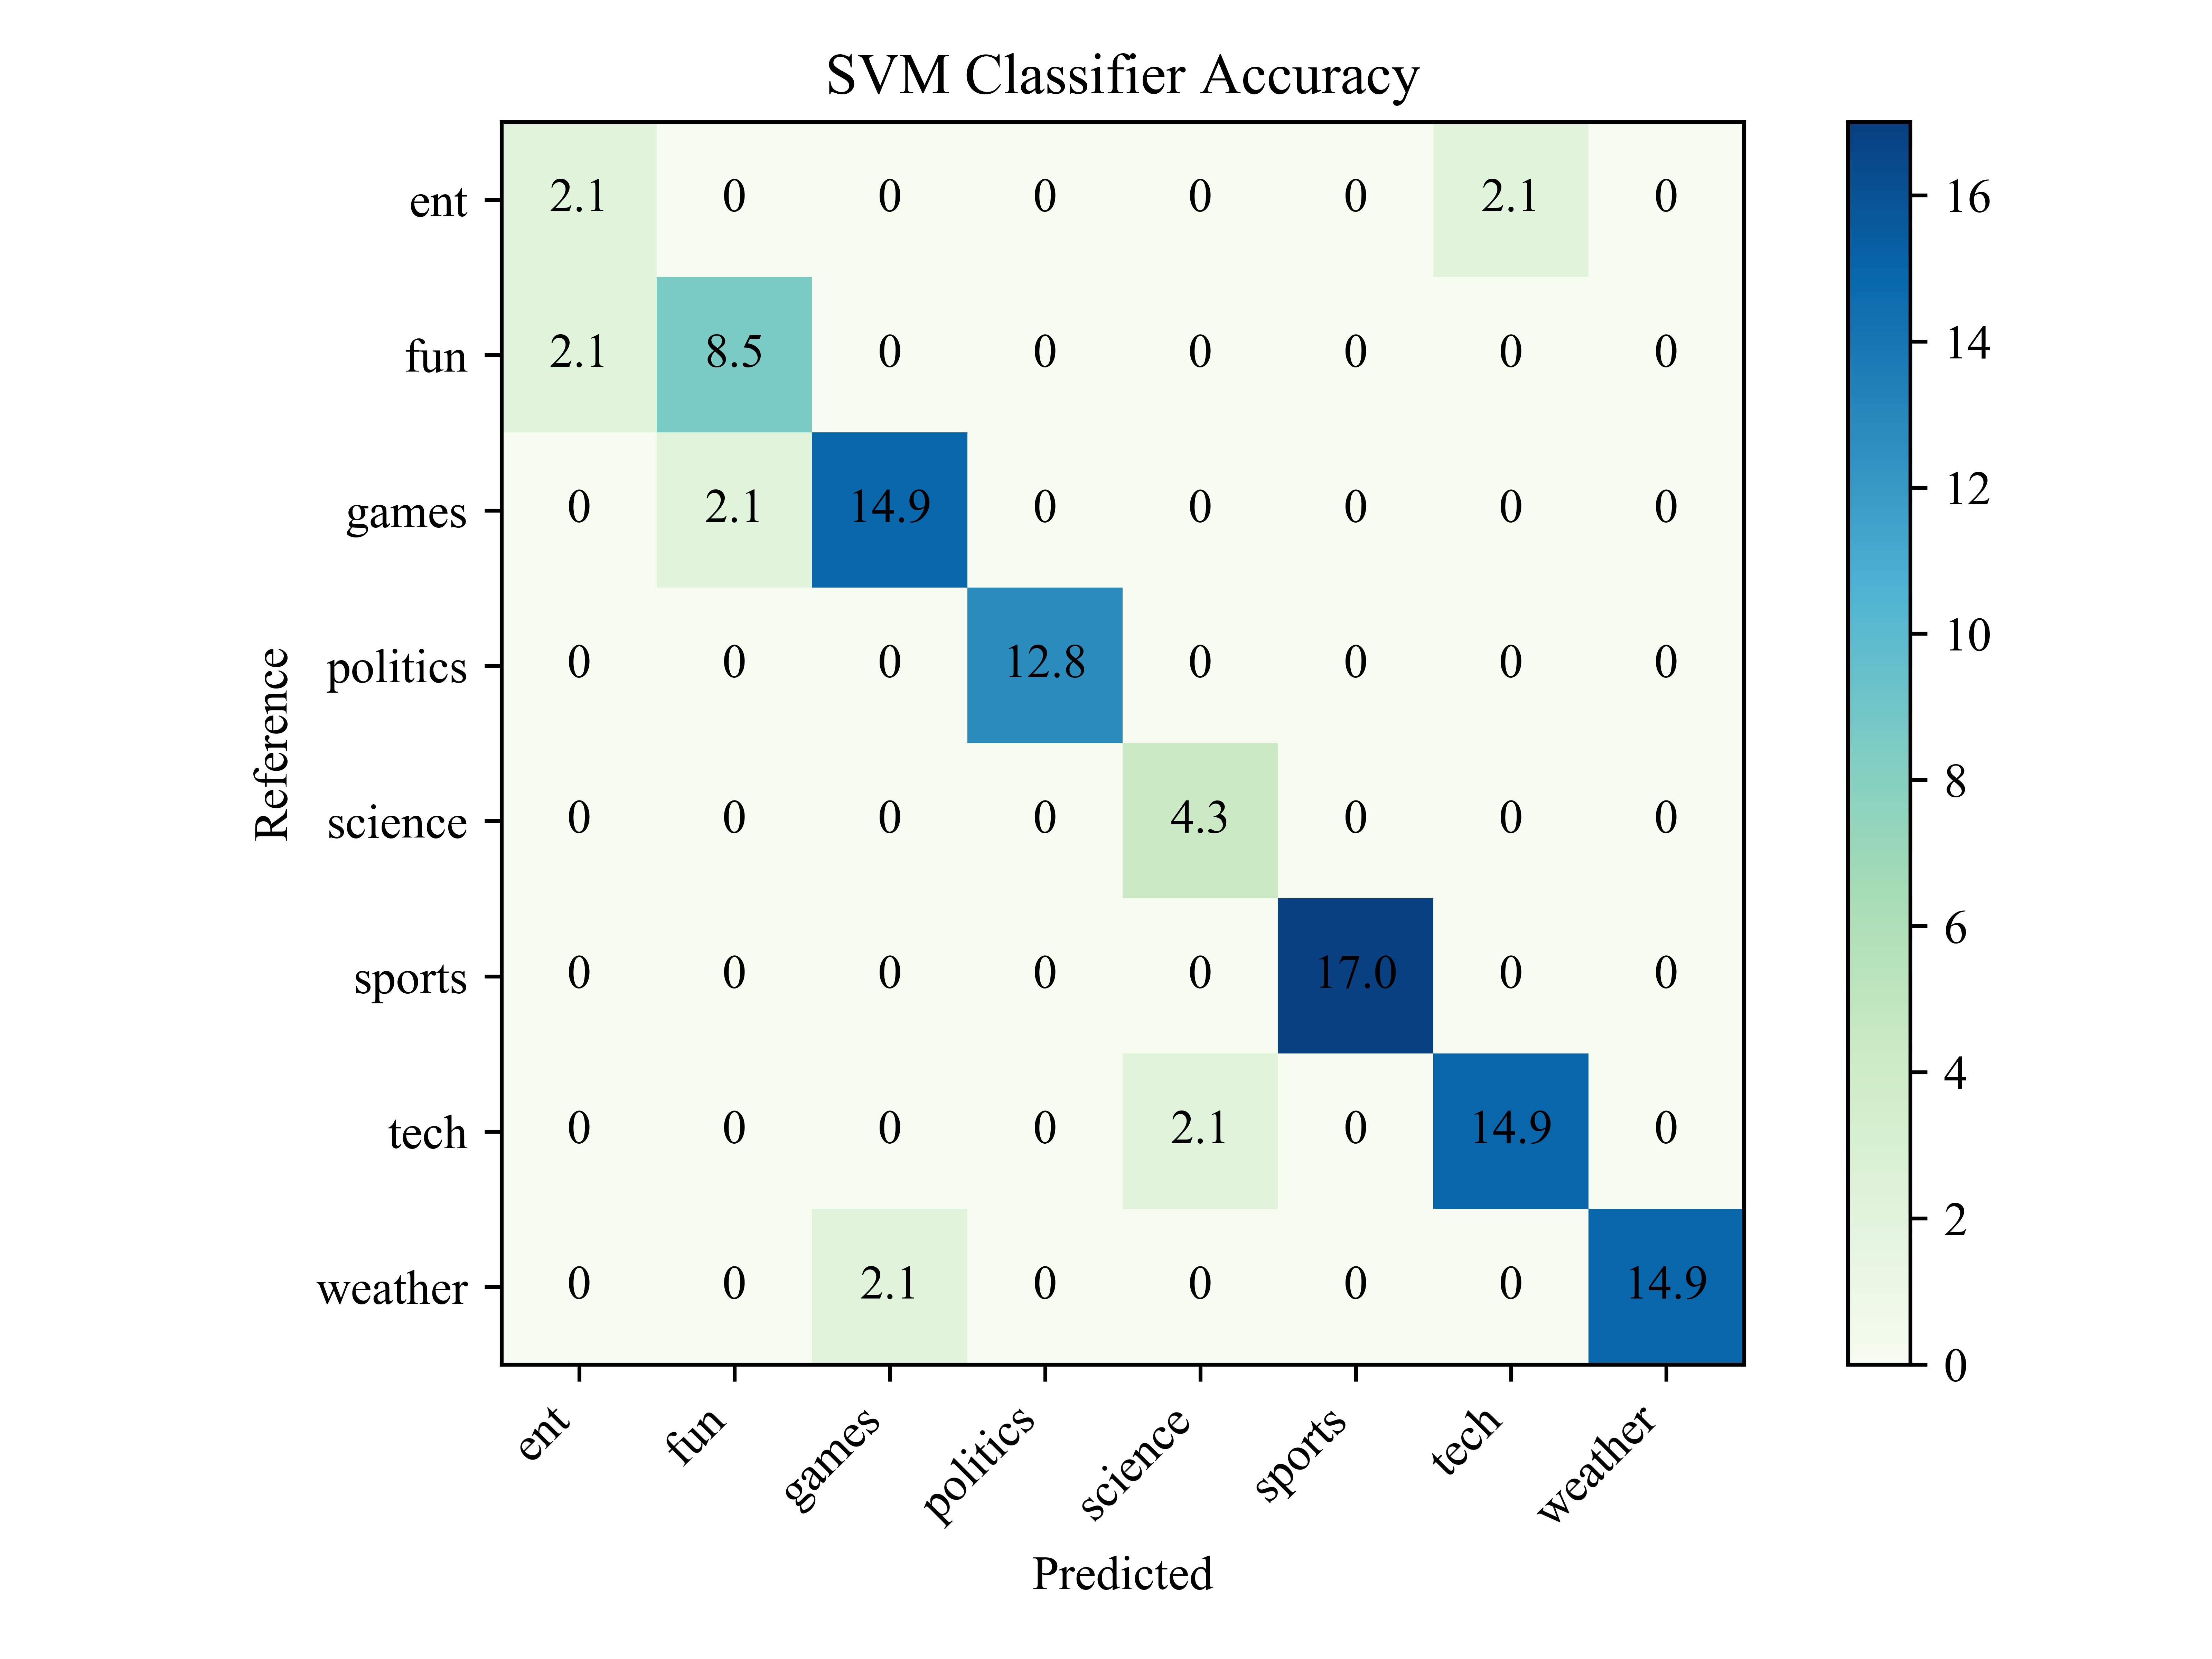
\includegraphics[width=8cm]{svm_cm}
    \caption{SVM Confusion Matrix}
\end{figure}

\begin{figure}
    \centering
    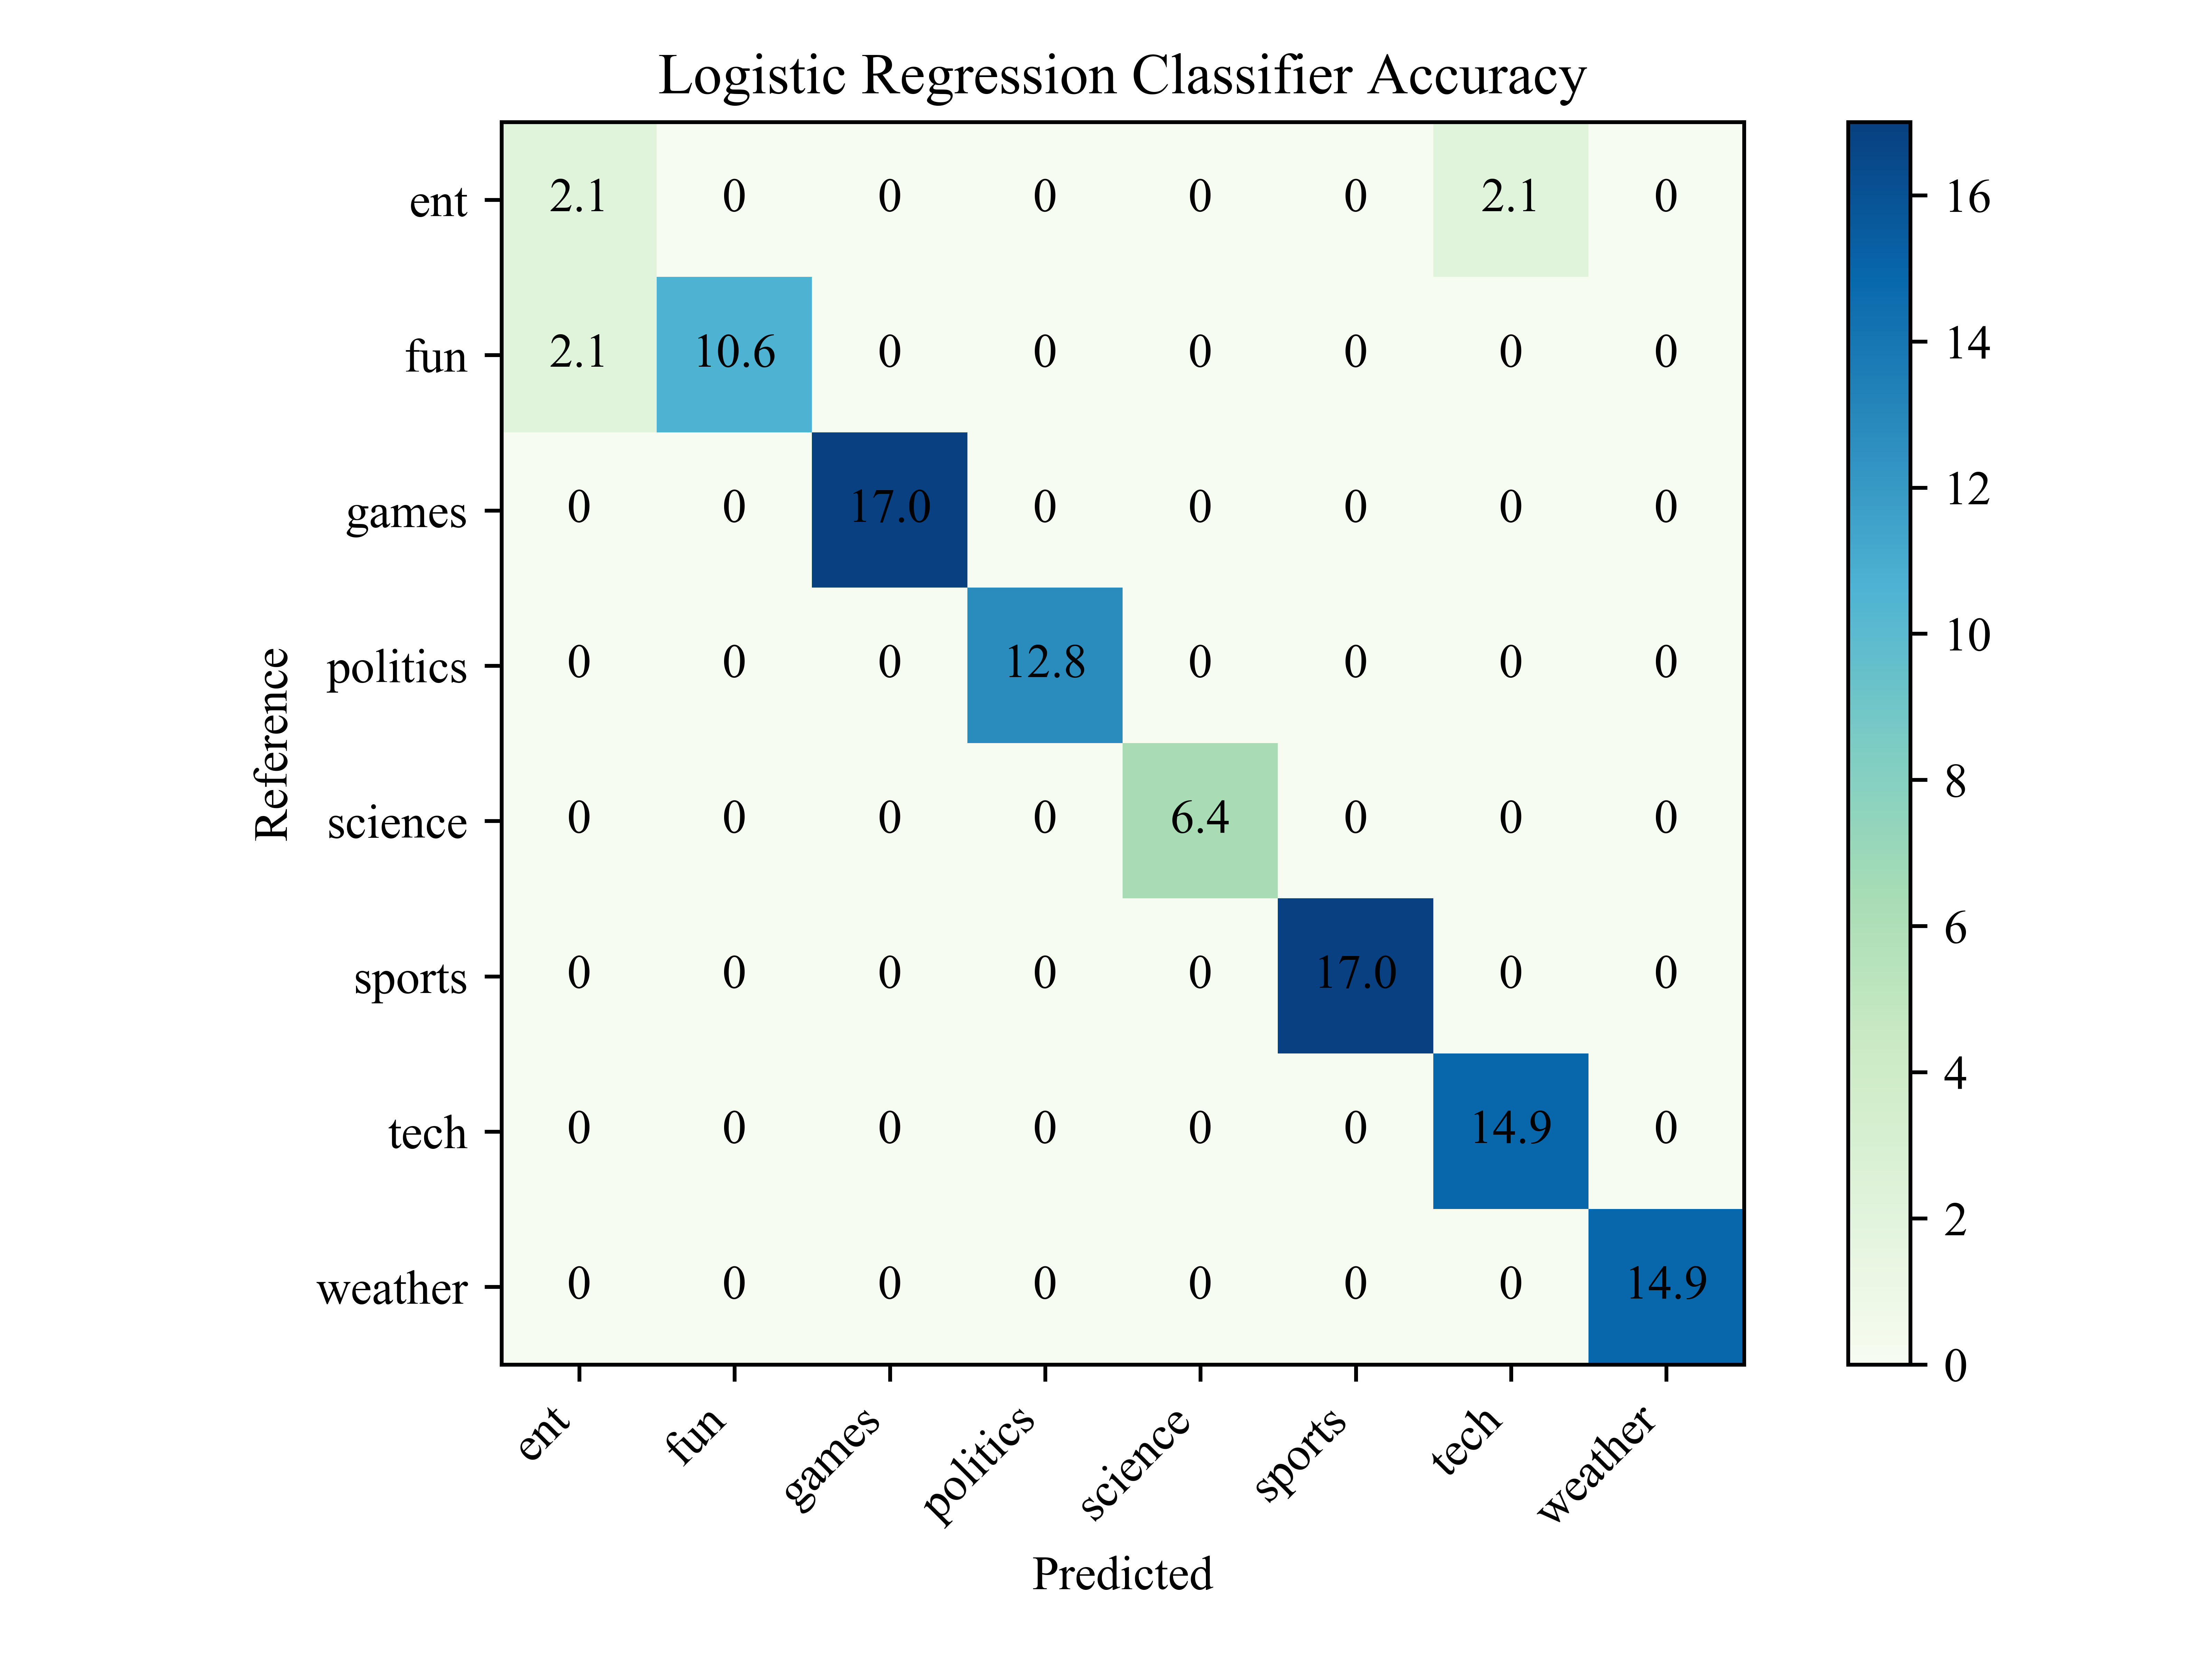
\includegraphics[width=8cm]{lr_cm}
    \caption{Logistic Regression Confusion Matrix}
\end{figure}

In general, the classifiers were able to pick up tweets that had highly informative features. For instance, a tweet mentioning ``Michael Jordan'' was more probable to be a sports tweet than a weather tweet. Examples of a politics, entertainment, and sports tweet with such features are listed below:
\begin{itemize}
    \itemsep 0em
    \item \texttt{"House Speaker Paul Ryan: "We're listening to our members" on the health care bill" -- CNN}
    \item \texttt{".@Syfy's \#TheExpanse is officially renewed for Season 3" -- Variety}
    \item \texttt{"Bulls x Celtics. Now. Watch live on ABC or here" -- ESPN}
\end{itemize}
In the majority of cases, the classifiers made two types of errors -- either the tweet was too short or it contained misleading features. For the first type of error, tweets such as ``must have wine'' were difficult to categorize because they did not have features that drove the classifier towards one category. Because our processing requirement enforced a minimum length of three words, tweets like the one above passed the test, but ran into numerous problems during classification. This problem could potentially be solved by increasing the minimum length requirement, but it would have the side effect of decreasing the overall corpus size.

The second type of error was much more difficult to diagnose. Take the following tweet, for example: \texttt{"i bet at least one person in the bbc newsroom psychically cracked their belt when they heard about the shift in northern ireland." - alicewhitey}. This tweet contains words such as ``bbc,'' ``newsroom,'' and ``ireland,'' which probably lead the classifier to believe it was politics-related. However, this tweet was in the fun category, and intuitively, this makes sense. Politics tweets are usually more formal and, for the most part, have correct spelling, grammar, and punctuation. This tweet, on the other hand, is informal and entirely in lowercase. This difference is much subtler, so this problem would require extracting different features.

\section{Future Work}

There were many problems we encountered as well as approaches we did not take that could be addressed with further research. First, computational power was the biggest bottleneck that prevented us from considering other qualitative features. We could barely train our classifiers with bigrams, as converting sentences to bigrams and ranking said bigrams with statistical tests took quite a while. We attempted to use other ngram models as feature sets for the classifiers, but this was not feasible given our computational constraints.

Second, we could consider other features, such as emojis, or quantitative features such as the number of punctuation marks, capitalized words, or spelling errors. Including these features could inform the classifier on top of our existing features. For instance, we noticed that the Olympics often had tweets consisting of sports-related emojis, such as soccer balls and footballs. Emojis are essentially a visual extension of our language, so taking these into account would surely aid classification. Further, as shown in alicewhitey’s tweet in the Error Analysis subsection, non-capitalized words were features that should have been considered. Including these types of quantitative features could give the classifiers a different perspective on the information contained in tweets.

Third, the NLTK \texttt{UnigramTagger} used in the POS feature set preparation was not that accurate. We can look into using the \texttt{BigramTagger} or the \texttt{HMMTagger}, which take more time to train but are proven to be more accurate. Further, the \texttt{UnigramTagger} was trained on the Brown Corpus, but other corpora such as the Penn TreeBank could also be used.

Finally, we can expand the number of categories we currently use to classify tweets. Twitter itself clusters its users around other domains, such as music, lifestyle, academics, and nonprofits, so these can be included in a future version of the corpus.

\printbibliography

\end{document}
